\documentclass[11pt]{article}
%Gummi|065|=)

\title{\textbf{Convertidores CC-CA y convertidores CD(Cc-Cc)}}
\author{Briano García Angel Eraclio\\
		Circuitos electronicos de interfaz\\
		Ing. Mecatrónica 4°B}
\date{17 de Septiembre del 2019}
\begin{document}

\maketitle
\newpage

\section{Estructuras básicas (sin aislamiento)}
\subsubsection{Reductor (Buck)}

Convertidor, reductor o buck destaca por su fácil manejo y su elevado rendimiento. Es el mas
fundamental de los convertidores CC-CC. Permite un rizado bajo de la tension de salida, y
es facil de estabilizar cuando trabaja en lazo cerrado, y permite una facil proteccion frente a
cortocircuitos y de limite de corriente.\subsubsection{Reductor-Elevador.}
Es un tipo de convertidor DC-DC quentiene una magnitud de voltaje de salida que puede
ser mayor o menor que la magnitud de voltaje de salida que puede ser mayor o menor que la
magnitud de voltaje de entrada.
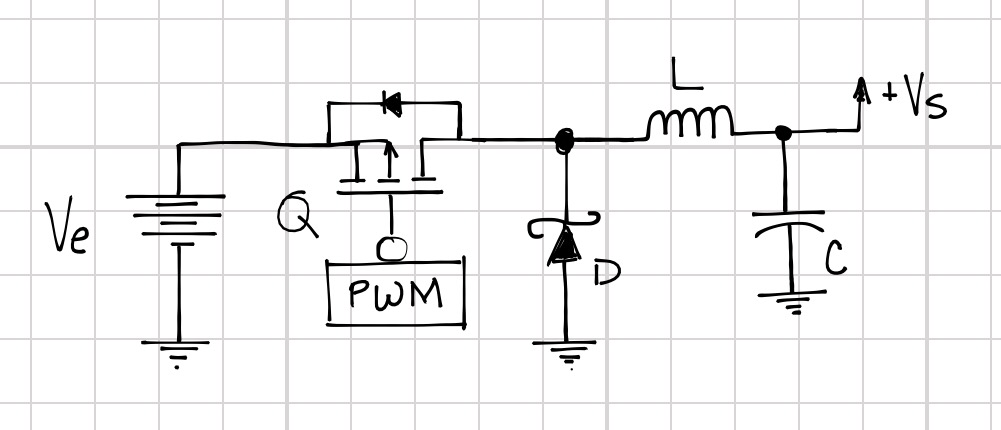
\includegraphics[scale=1]{imagenes/img_0365.png} 
\subsubsection{De Retroceso (flyback)}
Convierte los pulsos de alto voltaje en corriente continua que
luego el condensador formado en el TRC, filtra o plana. El alto voltaje puede desarrollarse
directamente en un solo bobinado con muchas espiras de alambre, o un bobinado que genera
un voltaje mas bajo y un multiploicador de voltaje de diodo condensador.
\subsubsection{Flyback 2 interruptores}
Cuando el interruptor esta activado la bobina primaria esta conectada directamente a la
fuente de alimentacion. Esto provoca un incremento del flujo magnetico en el nucleo. La tension
en el secundario es negativa, por lo que el diodo esta en inversa.
\subsubsection{Convertidor de Cuk}
La configuracion basica del convertidor de cuk se deriva de la operacion en serie de las
configuraciones basicas tipo boost y buck. Este convertidor, como todo convertidor CC-CC
presenta los dos modos tipicos de funcionamiento, conocidos como modos de funcionamiento
ininterrumpido y discontinuo. Es un tipo de convertidor DC-DC en el cual la magnitud de
voltaje en su salida puede ser inferior o superior a su voltaje de entrada.
\subsection{Estructuras de 2 y 4 cuadrantes sin aislamiento}
\subsubsection{Reversible de corriente}
El convertidor push-pull trabaja en el primer y tercer cuadrante. Es decir, el transformador
se magnetiza y se desmagnetiza en un periodo de trabajo. Esta compuesto por un tipo de 
inversor que convierte la tension continua en alterna utilizando dos transistores y un rectificador
de onda completa y un filtro paso bajo.
\subsubsection{Puente completo}
El puente rectificador de onda completa es un circuito electronico utilizado en la conversion
de una corriente alterna en continua. Esta formado por 4 diodos. Si
el voltaje es positivo y mayor que el voltaje en directa, el diodo conduce. El
voltaje en directa de un diodo de silicio esta sobre los 0.7V. Si el diodo esta polarizado en inversa
no conduce. Gracias a esto se puede generar dos caminos del puente rectificador de onda
completa. Uno para la primera mitad del periodo, que es positiva y otro para la segunda, que
es negativa.
\subsubsection{Reversible de tension}
Es un circuito electronico que generalmente se usa para permitir a un motor electrico DC
girar en ambos sentidos, avance y retroceso. Son ampliamente usados en robotica y como puente
completo.
\subsection{Directo (forwar)}
El funcionamiento de forward se obtiene apartir del troceador reductor (buck) de un cuadrante. El funcionamiento hacia adelante y hacia atras del motor se puede obtiene intercambiando cualquiera de sus dos terminales. En el circuito,solo un contactor debe estar cerrado mientras el otro esta
abierto.
\subsection{Elevador Boost.}
Es un convertidor DC a DC que obtiene en la salida una tension continua mayor que en la entrada. Tiene al menos un elemento para almacenar energia.
\section{Convertidores Cc-CA}
\subsection{Segun su numero de fases}
\subsubsection{Monofasico}
\textbf{Semipuente:}
La tension maxima que deben de soportar los interruptores de potencia: UB, mas las sobretensiones que originen los circuitos practicos. La tension maxima en la carga UB/2.

\textbf{Puente completo:}
El inversor en puente completo esta formado por 4 interruptores de potencia totalmente
controlados, tipicamente transistores MOSFET o IBGT.

\textbf{Push-Full:}
Tension maxima que deben soportar los interruptores de potencia: UB, mas las sobretensio-
nes que originen los circuitos practicos, que en este caso seran mayores debido a la inductancia
de dispersion del transformador. Solo utiliza dos interruptores de potencia y ambos estan referidos a masa.
\subsubsection{Trifasica}
\textbf{Estrella:}
Si los devanados de fase de un generador o consumidor se conectan de modo que los finales
de los devanados se unan en un punto comun, y los comienzos de estos sean conectados a los
conductores de la linea, tal coneccion se llama conexion en estrella.

\textbf{Delta:}
Los generadores o consumidores de corriente trifasica pueden conectarse no solo en estrella
si no tambien en triangulo o delta. La conexion en triangulo se ejecuta de modo que el extremo
final de la fase A este unido al comienzo de la fase B este unido al comienzo de la fase C y el
extremo final de la fase C este unido al comienzo de la fase A. A los lugares de conexion de las
fases se conectan conductores de la linea.
\subsection{Segun su forma de onda de salida.}
\subsubsection{Cuadrada}
La tecnica de modulacion o el esquema de conmutacion mas sencillo del inversor en puente
completo es el que genera una tension de salida en forma de onda cuadrada. La conmutacion
periodica de la tension de la carga entre + VCC y -VCC genera en la carga una tension con
forma de onda cuadrada.
\subsubsection{Semi-Cuadrada}
Para obtener este tipo de onda cuando la tension es positiva en la carga se mantiene S1
Y S2 conduciendo(S3 Y S4 abiertos). La tension negativa se obtiene de forma complementaria
(S3 Y S4 cerrados y S1 Y S2 abiertos. La tension nula se obtienen cerrando simultaneamente
los interruptores. Otra forma de obtener tension nula a la salida es manteniendo todos los
interruptores abiertos durante el intervalo de tiempo deseado.
\subsubsection{Modulados}
La idea principal es comparar una tension de referencia senoidal de baja frecuencia con
una senal triangular simetrica de alta frecuencia cuya frecuencia determine la frecuencia de
conmutacion.
\section{Convertidores de CA-CA}

\subsection{Variadores de CA.}
Es un sistema para el control de la velocidad rotacional de un motor de corriente alterna
(AC) por medio del control de la frecuencia de alimentacion suministrada al motor. La tension
o voltaje se hace variar a la vez que la frecuencia, a veces son llamados drivers VVVF
\subsection{Ciclo de controladores.}
Considerese un circuito alimentado y la carga se conecta un interruptor implementado como
un tiristor, el flujo de potencia transmitido a la carga puede controlarse variando el valor eficaz
de la tension aplicada a la misma. Un circuito de potencia de tales caracteristicas recibe el
nombre de convertidor de tension alterna.
\subsection{Convertidores matriciales.}
La conversion directa CA-CA por medio de conversiones matriciales permite modular la
tension, frecuencia y fase del sistema electrico trifasico a objeto de controlar el comportamiento
de la carga, y permitir la regeneracion de energia de la carga a la alimentacion principal.
\section{Controladores CA-CD}
\subsection{Controlados}
Es un circuito empleado para eliminar la parte negativa o positiva de una senal de corriente
alterna de lleno conducen cuando se polarizan inversamente. Ademas su voltaje es positivo.
\subsection{No controlados}
En los circuitos rectificadores se pueden sustituir total o parcial a los diodos por tiristo-
res, obteniendo un sistema de rectificacion controlado (formados unicamente por tiristores) o
semicontrolados (formados por tiristores y diodos). La puerta es la encargada de controlar el
paso de corriente entre el anodo y el catodo. Funciona basicamente como un diodo rectificador
controlado, permiendo circular la corriente en un solo sentido.
\end{document}
